\input{preamble}

\hypersetup{
  pdftitle={AAUB\AA D},
  pdfsubject={6th semester of Electronics and IT, Aalborg University},
  pdfauthor={Brian Bach Nielsen, Nick \O stergaard, Simon Als Nielsen, Rasmus Lundgaard Christensen and Christoffer Stagsted Andreassen},
  pdfcreator=LaTeX,
  linkcolor=black,
  citecolor=black,
  filecolor=black,
  urlcolor=black
}

\begin{document}

% Frontpage
\newgeometry{left=3cm,top=3cm,right=3cm,bottom=3cm}
\author{Nick Østergaard and Jeppe Dam}
\title{\textbf{\emph{Formation Control for Unmanned Surface Vehicles for Surveying Purposes}}}
\date{\today}
\maketitle
\thispagestyle{empty}
\begin{center}
	\includegraphics[width=13cm]{frontmatter/aauship}
\end{center}
\vfill
\begin{center}
	\includegraphics[width=5cm]{frontmatter/AAU_LOGO_CMYK_UK}\\
	Department of Electronic Systems
\end{center}
\clearpage
\restoregeometry

\frontmatter
\chapterstyle{nickoe}

%\layout
%  \includepdf{illustrations/cover}
%\cleardoublepage
%\input{formalities/titelbladdk}
\cleardoublepage
% Dette er LaTeX-versionen af titelbladet for tek-nat-basis-rapporter
% 2004 efterår Filen kræver: Universitetets logo: aau-logo.png (for
% LaTeX) eller aau-logo.ps (for LaTeX) Synopsis: En fil ved navn
% synopsis.tex

% Udarbejdet af: Hans Høttel (hans@cs.auc.dk) 21. maj 2003 Rettet af
% Morten Christophersen (mortench@tnb.aau.dk) 30. nov 2004(ændret til
% nyt design 2004 efteår) Modificeret af Nick Østergaard
% (noeste90@student.aau.dk) 28. sep 2009

\thispagestyle{empty}
\begin{flushleft}
%\begin{nopagebreak}
  {\samepage 
    \begin{tabular}{r}
     \fbox{ \parbox{\textwidth}{
       \raisebox{20mm}{\hspace{3cm}\includegraphics[width=3.35cm]{frontmatter/AAU_LAT_CIRCLE_blue_rgb}}
        \hfill \parbox{7cm}{
          \begin{tabular}{l}
            {\textsf{\small \textbf{Institute of Electronic Systems}}}\\
            {\textsf{\small \textbf{Control Engineering}}} \\
            {\textsf{\small Fredrik Bajers vej 7}} \\
            {\textsf{\small 9220 Aalborg \O st}} \\
            {\textsf{\small Phone 99 40 86 00}} \\
            %{\textsf{\small Fax 98 13 63 93}} \\
            {\textsf{\small http://es.aau.dk}}
          \end{tabular}}}}
      \\
    \end{tabular}

\begin{tabular}{cc}
\parbox{7cm}{
%\begin{description}

%\end{description}
\parbox{7cm}{
	\begin{list}{}{\leftmargin=0.5em}
	\item [\textbf{Title:}] \tightlist
	\item Formation Control for Unmanned Surface Vehicles for Surveying Purposes
	\item [\textbf{Theme:}]
	\item Master’s thesis
	\end{list}

	\begin{description}
	\item[Projectperiod:] \tightlist
	\item 2014
	\end{description}
	%  \hspace{4cm}
	\begin{description}
	\item[Projectgroup:] \tightlist
	\item 1034
	%  \hspace{4cm}
	\end{description}

	\begin{description}
	\item[Participants:] \tightlist
	\item Nick \O stergaard 
	\item Jeppe Dam
	\end{description} 
	\begin{description}
	\item[Supervisor:] \tightlist
	\item Jesper Abildgaard Larsen
	\end{description}
	}
	\begin{description}
	\item[Number of printed copies:] ??
	\item[Number of pages:] \arabic{lastsheet} 
	\item[Appendices:] ?? + 1 CD
	\item[Finished on:] \today
	\end{description}
	\vfill 
} &
\parbox{7cm}{
  \vspace{.15cm}
  \hfill 
  \begin{tabular}{l}
  {\textbf{Synopsis:}}\bigskip \\
  \fbox{
    \parbox{6.5cm}{\bigskip
     {\vfill{\small \input{frontmatter/synopsis}
     \bigskip}}
     }}
   \end{tabular}}
\end{tabular}}
%\\ \\

\strut \vfill
%\noindent{\footnotesize\textsf{\emph{Rapportens indhold er frit tilgængeligt, men offentliggørelse må kun ske efter aftale med forfatterne.}}}
%\end{nopagebreak}
\includegraphics[width=1.35cm]{frontmatter/ca-logo.pdf}
\end{flushleft}

%Rapporten skal afleveres til følgende:
%1 stk. til hovedvejlederen (afleveres til studiesekretæren)
%1 stk. til censor (afleveres til studiesekretæren)
%1 stk. til hver studerende i gruppen

\chapter{Preface}
This is a master thesis concerning the platform named AAUSHIP. This platform is an ongoing project which have Jesper Abildgaard Larsen in charge. The first steps of the AAUSHIP project started in year 2011, where in the early stages had no intend to be a USV. The project have developed into the AAUSHIP platform, which is a USV in working progress. In this thesis have Jeppe Dam and Nick Østergaard been focusing on upgrading the hardware of the platform to overcome implementation errors, designing a applicable model of the platform and designing formation control strategies for a future fleet of AAUSHIPS for surveying purposes. The idea of surveying have been in focus for some time in the project, from where an initial correspondence between AAU and Aalborg Havn has been created. Aalborg Havn has the interest in the AAUSHIP project since they have an aim to become an intelligent harbour, and the work of this project is a stepping stone for them. On the basis of this have the surveying purpose in the Limfjord become the area of interest, which have given rise of directing the AAUSHIP to this purpose.

The work in the project have both given the project group an insight of the hardware issues at the AAUSHIP, but have also given rise to investigate the formation control aspects when dealing with groups of USV. Since the early work on the AAUSHIP project only have been on a single ship, the need for internal communication have not been crucial. Now, to upgrade the platform, the ROS system have been implemented both for future work but also for testing purposes behind the desk. This have given the group the opportunity to simulate the behaviour of the AAUSHIP in a controlled designed environment, and afterwards implement and realize the design on the AAUSHIP.
\newpage

\subsubsection*{Thanks to}
\begin{description}
\item[Karl Damkjær Hansen] has been glad to answer ROS related questions, which have proven very useful when redesigning the AAUSHIP to be handled through ROS. For future implementation to the AAUSHIP fleet will his knowledge with ROS also be of importance.\\
\item[Aalborg Havn] has been willing to share data, information and experience with surveying applications, and have shown interest in the project. As the state of the project is not fully worked out, and the AAUSHIP in a platform in progress, the direct corporation with them has not reached the implementation phase with their system yet. Though have their experience with surveying proven helpful. 
\end{description}


\begin{center}
  \begin{minipage}[t]{0.47\textwidth}
    \centering \vspace{1.5cm} \hrule \vspace{1mm} Nick \O stergaard
  \end{minipage}
  \hfill
  \begin{minipage}[t]{0.47\textwidth}
    \centering \vspace{1.5cm} \hrule \vspace{1mm} Jeppe Dam
  \end{minipage}
\end{center}


\newpage
\section*{Reading Guide}
The following report is divided into parts, related to different phases of the project. The parts are divided into chapters, the chapters describe different aspects of the project. The chapters are subdivided a number of times to further split up the content into specific topics. The report is ended with an appendix part, that contains all the material that is relevant to the project, but not necessarily interesting to the reader, such as measurement journals and transcripts of meetings.

\begin{description}
\item[Citations] in the report is done according to the Harvard method, the list of references can be found \vpageref{ch:litt}. The elements on the list of references are sorted by author.
\item[Acronyms] are written to their full extend, the first time they are used, with the acronym in parentheses, thereafter only the acronym is used. The list of acronyms can be found \vpageref{ch:acronyms}.
\item[Notation] of vectors are written in bold font with lower case letters ($\vec{v}$), matrices are written in bold font with upper case letters ($\vec{M}$). Single variables and constants are typeset in normal math ($x$).
\item[Attached] to the report is a CD, which contains copies of web references and other digital files (source code, scripts and raw measurement data) that could be of interest to the reader. In some places in the report there will be a reference to the CD; this will look like this: \cd{/path-to-file}.
\end{description}


%%%%%%% Maybe we should have an overview of the system here
\cleardoublepage
\tableofcontents
\chapter*{List of acronyms}
\label{ch:acronyms}
\begin{acronym}[TDMA]
  \acro{AAU}{Aalborg University}
  \acro{ABS}{Acrylonitrile Butadiene Styrene}
  \acro{ARGO}{Autonomous Research and Geo-Survey Oceanographer}
  \acro{ECEF}{Earth-centred Earth-fixed}
  \acro{GPS}{Global Positioning System}
  \acro{IMU}{Inertial Measurement Unit}
	\acro{MIMO}{Multiple-Input Multiple-Output}
	\acro{PWM}{Pulse-Width Modulation}
  \acro{RTK}{Real Time Kinematic}
	\acro{SISO}{Single-Input Single-Output}
  \acro{TCP}{Transmission Control Protocol}
  \acro{WGS84}{World Geodetic System 84}
\end{acronym}

%WRITE THE ACRONYMS ALPHABETACALLY!


\mainmatter
\descpart{Introduction}{In this part is the motivation for the project stated and the previous work within the subject will be summed up.}
\chapter{Introduction}
% \section{Introduction}

\cite{12gr730}

Lorem ipsum \acl{ASV}

\section{General formation control}
\head{This section will give a short introduction to formation control in general followed by some of the individual assignments which needs to be determined before the process of design can be started.}

%\head{Formation control in general is concerned with simultaneous control of dynamic systems. These systems is often referred to as agents where the objective of these is to maintain a static reference to a specified object. This object could be another agent witch then would be referred to as the leader. The other agents objective will then be to stay in the relative position to the leader within a static formation.}


The theory of formation control in general is widely applied. It is usually applied in assignments regarding control of robots which needs to be placed relative to each other. Depending on the given task of the robots, and which type of robots are in focus, the formation can be utilized in different ways.

The robots can also be of various types: Driving vehicles, helicopters, aeroplanes, ships etc. which can both be manned and unmanned. The tasks that these robots needs to fulfill can vary a lot and be both as individuals in a formation or as a whole group. Swarm robots in general got many purposes such as vacuum cleaning robots, who needs to clean a rather large area or flying robots like quadcoptors who can make different kinds of assignments. When quadcoptors work as a combined group they could lift a certain amount of payload to achieve their goal as a group, or they could work individually in a network to do several smaller tasks. An example of how quadcoptors are working together can be examined at \citep{ethswarm}.

All these robots are in the terminology called \textit{agents}. These agents move either individually or in formation. This formation can be rigid or be flexible. If the agents move in rigid formation they will keep their relative positions to each other and does not diverge from the formation. The formation could also be flexible which sometimes proves to be preferable. If the distances between three agents on line are large, and an obstacle needs to be avoided, only one of the agents needs to move from this obstacle if the formation is flexible. This can be seen on figure~\vref{fig:form_avoid_right}. \todo{Inddel i afsnit, sådan mere generelt over det hele}
\begin{figure}[htbp]
	\centering
	\includesvg[width=0.5\textwidth]{form_avoid_right}
	\caption{A flexible formation where the right agent avoids an obstacle.}
	\label{fig:form_avoid_right}
\end{figure}

\section{State of the art}
When looking into formation control many different types of control can be taken into control. The main types of formation control are separated into six different types, separated by \cite{muv-survey}, all under the main topic \textit{multiple vehicles coordination strategies}. The overview for this can be found in the survey paper \cite{muv-survey} who explains the six main types and a few alternations of these.

The theoretical views on control of \ac{MUV}'s behaviour are divided into two classes; centralized and decentralized systems. If the system is centralized this means that all control of the formation is done on one agent, and the others receive information from the core agent. This form of system has the advantage that the core agent can optimize vehicle coordination, accommodate individual agent faults and monitor the accomplishment of the mission. The main disadvantage of this system is that if a fault should occur in the core agent this will affect and facilitate a failure of the whole system.

The opposite way of controlling the system would be in a decentralized way. This way of controlling the formation is inspired by the aggregation of birds and fish. This makes each agent able to communicate and share information in between. This means that each agent is given its own part of the complete mission and thus can only complete a part of the mission. The advantage is that faults in a single agent can be overlooked, thus more robust to faults, but can result in a less efficient mission outcome. A decentralized system may be more appropriate to scale up such that more agents can be included and the computational load can, in difference from the centralized system, be split up onto more agents.

The different types of coordination and control algorithms within centralized and decentralized systems include: \textit{behavioural-based}, \textit{virtual structure}, \textit{leader-follower}, \textit{graph-based} and \textit{potential field approaches}. Within these structures are the terms Cooperation Control and Formation Control used. Cooperative Control focuses on the global task that the group of agents needs to fulfil, and the Formation Control is the actions performed by each agent which is shared with the other agents in the group. 
\begin{description}[style=nextline]
	\item [Virtual structure]
	In a virtual structure is the entire formation treated as a single entity. The behaviour coordination for a group of agents in a virtual structure is uncomplicated compared to the coordination of many agents, thus makes this the advantage when doing virtual structure. The disadvantage falls on the centralization due to the structure treated as a single entity. If a failure in this structure happen results in a failure in the entire structure.
	\item [Behaviour Based Methods]
	The behavioural based model employs several behaviours for each of the agents and the final control used to control the formation is derived from a weighting of the relative importance of each of the behaviours. This could for instance be navigational behaviours to enable a navigation to be the main goal while avoiding hazards and stay in formation. So if one agent needs to avoid a collision with an obstacle should the rest of the group not take this into account. Only that single ship needs to leave the formation and get back into formation again.
	\item [Leader-Follower Approaches]
	Applying leader-follower methods designates one agent as being the leader and the rest of the agents as followers. The following agents need to position themselves relative to the leader and maintain a desired relative position to the leader. This makes the simplicity to this method, but there is no feedback from the followers to the leader and thus makes that a disadvantage. Within leader-follower methods it is possible to enable changes in the shape of the team. Separation-separation and separation-bearing are two popular leader-follower formation controls, where the followers stay at specified separation and bearing from their designated leader. Within this method it is possible to split the group up into several smaller groups with their individual designated leader.
	\item [Potential Field Approach]
	Potential field approaches assigns potentials to agents to make a weighting between them. This weighting could for instance determine the relative distances between the agents. This is usually used when following a virtual leader, such that this process is only made relative to the agents within the structure. This method can make ensure a collision free formation when every agent has been assigned their potential weighting respectively. In this method obstacles can be included and have assigned potentials as well. This will become a avoidance radius from the specific object.
	\item [Graph Theory Approaches]
	When applying the graph theory method one assign every agent as a node and assign connections between the nodes. In graph theory this is denoted vertices and edges. The study with graph theory is mainly concentrated of the formation itself and related to changes within the structure. This can be related to the structure within a tree-structure which is used when assigning the formations in graph theory manor. This can be applied as communication analysis for the agents and consensus analysis can be of benefit. The edges between the nodes symbolizes the possible connections thus communication between them. The nodes that are connected are denoted as neighbours and are capable of communicating.
\end{description}

\section{Motivation and the AAUSHIP project}
These above mentioned theories makes the basis for the formation control within the scope of this project. This thesis will utilise formation control and extensions to manoeuvre agents through a specified area.

The port of Aalborg would like Aalborg University to help them to expand their options of improving the conditions of the Limfjord. One of their tasks is to map the seabed of the Limfjord. This would be preferable when they want to improve the conditions of the Limfjord. The port of Aalborg wants to make of a profile of the slopes of the channel in the Limfjord. This will help them guide larger cargo ships to port while using the autonomous ships as guidance.

Another aspect from the port of Aalborg is a task to escort larger ships with cargo into the port of Aalborg. This is done by a pilot whom needs to sail out to incoming larger cargo ships and escort them safely into port. The pilot does this in a pilot boat which is controlled manually by the pilot. The port of Aalborg would like this process to become autonomous such that an autonomous boat can sail to the cargo ship and to some extend take over the control and guide the cargo ship into port. The system to do this implies that the port of Aalborg needs an autonomous ship which can perform this task.

The mapping itself can be done by one ship or by more. For the moment one of the ships from the port of Aalborg, which is manned, and covers the mapping of the closer part of the Limfjord ($\approx$ 65 km). This is only done every third year, but mapping around Hals Barre (a sandbar \todo{slet efterfølgende kommentar igen engang}and not a beach bar) at the end of the Limfjord is a more critical place and is mapped every third month.

If the port of Aalborg had admitted an autonomous ship, which could sail out and do the mapping by itself, t ey would see to map the outer part of the Limfjord more often to be able to deliver more precise seabed mappings to incoming ships. Due to the autonomous system with boats would the port be able to take measurements more often of the complete fjord and therefore more favourable than only having measurements each third year. \cite{portofaalborg}.

\subsection{The mission}
Within the scope of this project the robots will be unmanned ships,
\ac{ASV}. The ship's main purpose will be to map the seabed by using
sonars. When one ship need to do this alone, and due to the range of
the sonar, the time spend could be improved. The sonar scanning would
be done as seen on figure~\vref{fig:concept-art}.

\begin{figure}[htbp]
	\centering
	\includegraphics[width=0.48\textwidth]{fig/conseptart-single}
	\includegraphics[width=0.48\textwidth]{fig/conseptart-formation}
	\caption{Concept drawings of ship scanning a sea floor. Left is a
	single ship, right is a fleet of ships in formation.}
	\label{fig:concept-art}
\end{figure}

When only one ship need to map a complete seabed this process could
take up much time dependent on the area that need to be covered. The
time spend could be improved to make this mapping more efficient. One
way of optimizing the time used is to add more ships to help map the
seabed. To make the process of this as optimal as possible it could be
of benefit to implement formation control in the specific assignment.
This could be done in several ways, but is mostly thought of in a
rigid formation, such that the formation maps the same area of the
seabed the whole time. The idea can be seen on
figure~\vref{fig:concept-art}.

The distances between the ships would be determined by how far the sonars could reach the seabed. There should be some overlap of the maps from each sonar but still as little as possible. The specific formation could be a simple line or it could be more advanced formations. This does not have any relevant impact of how the mappings of the seabed would be due to the subsequent processing of the collected data from the maps. Different formations of ships can be seen on figure~\vref{fig:diffforms}.
\begin{figure}[htbp]
	\centering
	\includesvg[width=0.5\textwidth]{diffforms}
	\caption{Different formations which the \ac{ASV}s can make.}
	\label{fig:diffforms}
\end{figure}
The formation of the ships may not need to be strictly rigid. Situations could appear where it would be of benefit to change the ship's formation. If the formation need to avoid an obstacle and one or more ships needs to go faster or slower, which leads to a change in the formation, it might be of benefit to regroup the formation which is faster to reach. An example can be seen on figure~\vref{fig:avoid}.
\begin{figure}[htbp]
	\centering
	\includesvg[width=0.5\textwidth]{form_avoid}
	\caption{A formation needs to go around an obstacle where the inner most ship chooses the shortest path and the formation regroups.}
	\label{fig:avoid}
\end{figure}

When doing the formation control it is important to figure out what one
want to achieve, and depending on the strategy and the formation type
some things are to be considered as requirements regarding how the
formation should work. In this discussion lawnmower patterns are considered. In this work two ships are considered for simplicity, but it should be extensible to n-number of ships. The lawnmower patterns will suit well for the mapping of a seabed where one or more ships are to sail from shore to shore in a fjord.

When looking at the specific task several things needs to be taken into account. When starting the mission, the ships may start at positions that is not in the desired formation. It might be of importance that the ships are in
formation when they start tracking the desired track. Therefore some
attention must be given on how to make the ships initialize this
formation. This is referred to as the group coordination task. An approach is to make the ships sail individually to the
starting positions with a speed that makes them hit their respectively starting points at
the same time. If one reaches its start point much earlier
than the other it must stop, which is not wanted because it then can
drift out of position again. This basically means that there exists an initialization
phase and a tracking phase. The start heading should of
course align with the path at the start point such that the path following can begin with zero error. The ships could also target their group formation before starting at time zero at the path. This will eventually make the initialization take longer time but ensure that the ships have made the group coordination task and are ready to start at the path.

Another issue to be considered is to ensure that no ship at
any point in time reaches a minimum speed that is necessary for the
ship to not drift out of formation. This could be a problem in corners
of the formation if a stiff construction, where the inner most ship
has to move slower, to accommodate the shorter distance on an inner
circle arc.

Faults like blackout on a ship could also be considered in the control
design. I.e. what happens with the formation when one ship faults in a
blackout. Should the rest of the formation stop, should the formation
still follow this drifting ship or should the mission simply terminate
when it is discovered that a ship has blackout. This is under the assumption that the formation is decentralized and every ship has its own control and is not controlled from a mother ship.

In the initialization phase it is also relevant to consider how the
ships should avoid each other if they are on the wrong side of each
other. If it is of benefit that a specific ship is at the most inner route, and is located at an outer position before the group coordination, this ship needs to cross the formation to get to the desired starting position. This initialization needs to be adjusted in the initialization phase to ensure that no ships collide.

\begin{figure}[htbp]
	\centering
	\includesvg[width=0.4\textwidth]{cornoring}
	\caption{Two ships initializing and following the path offset
		equally on each side, ships are constrained to sailing parallel
		and heading the same as path when projected onto the path. Blue
	dot is start of path. Fully drawn splines is initializing phase.}
	\label{fig:cornoring}
\end{figure}

On figure~\vref{fig:cornoring} is a simple path following performed
with two ships in a stiff formation with an equal distance from the
path. It illustrates four steps. In step \#0 the ships initializes a
random position near the start of the path being the group coordination task. At \#1 it is tracking the
path in formation, whilst still in formation. This is referred to as a formation coordination task. At \#2, the green
(right) ship is in a tight inner curve where it is important to
consider design of the path such that the capabilities of the ship is not
exceeded to stay in formation. At \#3 it is back to straight line path
following in formation. \citep{thorvaldsen}.

\begin{figure}[htbp]
	\centering
	\includesvg[width=0.6\textwidth]{form_rigid_90}
	\caption{Three ships in formation needs to make a 90\textdegree turn and stays in their relative positions and keeps the rigid formation.}
	\label{fig:form_rigid_90}
\end{figure}

When the ships needs to make a turn about something they can do it in many ways. On figure~\vref{fig:form_rigid_90} the ships keep their formation whilst turning about the object. When they reach the other side and have finished their turn, the ships have kept formation but the outer most ship has now become the inner most ship. The reason to turn like this could be that the inner most ship, the yellow ship, cannot turn as sharp as demanded to stay the inner most ship. Therefore, instead of turning the formation, they stay geometrically rigid.

\begin{figure}[htbp]
	\centering
	\includesvg[width=0.6\textwidth]{form_change_90}
	\caption{Three ships in formation needs to make a 90\textdegree turn and changes their relative positions.}
	\label{fig:form_change_90}
\end{figure}

As seen on figure~\vref{fig:form_rigid_90} the ships could have benefit of turning like this. This way of turning could cause trouble in the top of the turn, where the ships eventually will collide due to errors and the relative close distance to each other. This way could be altered a little such that the ships will turn like on figure~\vref{fig:form_change_90}. There the ships adjust their position and velocities to ensure that they will not collide, but they will therefore leave their formation shortly to return back into position again.

\subsubsection{Degree of Actuation}
The degree of actuation is a matter that sets some limitations on how
the path following can be made, and thus the methods available to
control the ships.

AAUSHIP is a ship, which means that is is not fully actuated in the
whole 3D space, but this is not needed since it is moving on a
surface. To be fully actuated it must be able to have controls for
surge, sway and yaw.

There are different ways of controlling, and a few could be:
\begin{description}[style=nextline]
	\item [Three or more controls]
	When having three or more control parameters it is said that the vessel is fully actuated. This way of controlling is usually used in low-speed manoeuvring and stationkeeping mostly by offshore \ac{DP} vessels.
	\item [Two controls and Trajectory-Tracking control]
	Trajectory-Tracking is done in a three \ac{DOF} system, $e(t)\in\mathds{R}^2\text{X}S$. It is done with two control inputs, $u(t)\in\mathds{R}^2$. This means that the control problem is underactuated which cannot be solved by linear control theory. A vessel under these terms is able to manoeuvre along a path with constant sideslip angle using only surge and yaw. This is the classic approach for path following.
	\item [Two controls and Weather-Optimal heading]
	When taking the weather conditions, and in general the environmental disturbances, into account, it is done as a mean of all the disturbances. This is used to stabilize the vessel regarding the position. It is done by making the heading depend of the change in the mean of the environmental disturbances.
	\item [Two controls and Path-Following control]
	The standard way by having two controls, being surge and yaw, and achieving path-following, is to define a 2-D workspace. This workspace is placed along the trajectory with along-track and cross-track vectors that are to represent the error to minimize. This is usually done by applying the \ac{LOS} path following controller that makes use of surge and yaw to accomplish the path following. This implies that a six \ac{DOF} system model needs to be internally stable such that only the two control inputs are used.
	\item [One control]
	This is only done with systems with three \ac{DOF} and is normally only used to stationkeeping.
\end{description}
\citep{fossen}

\subsection{Delimitations}
Within the scope of the AAUSHIP project will the focus be to apply and extend a leader-follower approach at the ships. This will include several tasks. The two main tasks will be to make a group coordination task and a formation coordination task. The group coordination task will be, as described earlier, an objective to get the ships into the desired formation before or exactly at the starting point of the path following. The formation coordination task will be to make a leader, virtual or not, follow a predetermined path set by waypoints. The path should be generated from waypoints placed on a map due to that the ship needs to travel over larger distances. This will make a waypoint based follower where the path will be generated between the placed waypoints.

The placement of the waypoints will be placed such that the ships need to surge along a lawnmower pattern, where the turns have a lower requirement of turn radius dependent on the surge velocity of the most inner ship. This is due to the drift if the inner ship looses too much velocity.

When applying the leader-follower approach it needs to be determined how the formation precisely should be set up. In this project is only one leader considered at a time. The rest of the ships will act as followers to the leader. The idea can be seen on figure~\vref{fig:l_f} where only one leader is represented with a single or more followers.
\begin{figure}[htbp]
	\centering
	\includesvg[width=0.6\textwidth]{lead_follow}
	\caption{A leader is always assigned and potential followers are following.}
	\label{fig:l_f}
\end{figure}
When the followers are in formation with the leader is only the leader who is following a specified trajectory. The other ships, the followers, only keeps their position relative to the leader. This makes the predetermined formation moving along the path relative to how the leader is following the path. The leader is autonomous as well as the followers, but the path following is only done at the leader and the followers maintains their relative positions to the leader.

If the leader diverges from the path, drifting to the left, this will result in the whole formation drifting to the left. This problem can be dealt with in different ways, e.g. the control could react fast enough to make the formation get back on track within a specified time, or some fault tolerance could be done from the whole system. If the leader diverges from the path it could make the formation stay at their respective headings within a time slot before actuating towards the leader.

The formation needs to take into account if it is of benefit to change leader. If some kind of obstacle makes the formation turn about it, it might come to benefit to change the leader which needs to be done on the fly. This entails a change in the group coordination and the ships needs to set their relative position and heading from another ship.

The configuration of the formation will be set up, as a start, with one leader and a single follower. The follower will be offset from the leader with a distance of five metres. This can be seen on figure~\vref{fig:l_f1}.
\begin{figure}[htbp]
	\centering
	\includesvg[width=0.4\textwidth]{lead_follow1}
	\caption{The leader with a follower offset by 5 metres radius.}
	\label{fig:l_f1}
\end{figure}
This will be a rigid formation that the ships needs to keep at all times. The change of leader will eventually be taken into account when the ships needs to turn. If the formation needs to turn clockwise about it might be of benefit to change the leader. 

The location to test and implementation the AAUSHIPs will be in the Limfjord. The optimum will be to make the formation go across the Limfjord and back in lawnmower pattern and make measurements of the seabed. Due to the location where it is presumed to have enough space, the formation is not of bigger importance to the mapping. The only important thing to include regarding the formation is that the ships needs to be able to turn around without loosing so much velocity such that they start drifting and offset the formation.


% \descpart{Preliminary analysis}{%
% This is da stuff that is roolin'.}

\descpart{Control Design}{}
\chapter{Different control strategies}

\section{Manoeuvring the vessel using the LOS method}
Path-following problems for vessels are often solved by implementing \ac{LOS} algorithms. Opposite to other position control algorithms, where the vessel may be driven both in longitudinal and transversal directions to converge to a path, the \ac{LOS} algorithm gives a more natural motion towards the desired path. This is done by giving a more natural reference to the heading of the vessel. One of the advantages of this is that it can be applied both to fully actuated and under actuated vessels.

Since it is only the leader, and not any of the followers, who need to follow a path, this is only applied on one vessel. This can also be extended to a leader in a virtual structure. To apply the \ac{LOS} algorithm a setup is needed. To get an overview of the functionality of the \ac{LOS} algorithm see figure~\vref{fig:allinallframes}.
\begin{figure}[htbp]
	\centering
	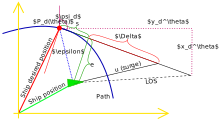
\includegraphics[width=\textwidth]{fig/allinallframes}
	\caption{A ship placed beside the path and uses the \ac{LOS} algorithm to get back on track.}
	\label{fig:allinallframes}
\end{figure}
\chapter{Modelling}
\head{Within this chapter will different models be developed to make the actuation of the vessel more precise.}

\section{Added Mass Modelling}
Definition: Hydrodynamic added mass is defined as the mass added to a system due to an accelerating or decelerating body must move a volume of the surrounding fluid as it moves through it. To this is said that the object and fluid is not able to occupy the same physical space simultaneously.

\section{Rigid Body Modelling}
The rigid body is used to model the physics of the vessel. It is an idealization of the solid body from where the physical motions of the vessel are to be derived. From analysis of this can translational motion and rotational motion be derived, and by \citep{fossen} written in component form as:
\begin{align}
f^b_b &= [X,Y,Z]^T & &- \text{force through } o_b \text{ expressed in } \{b\}\\
m^b_b &= [K,M,N]^T & &- \text{moment about } o_b \text{ expressed in } \{b\}\\
v^b_{b/n} &= [u,v,w]^T & &- \text{linear velocity of } o_b \text{ relative } o_n \text{ expressed in } \{b\}\\
\omega^b_{b/n} &= [p,q,r]^T & &- \text{angular velocity of } {b} \text{ relative to } \{n\} \text{ expressed in } \{b\}\\
r^b_g &= [x_g,y_g,z_g]^T & &- \text{vector from } o_b \text{ to CG expressed in } \{b\}
\end{align}

\section{Disturbances}


\subsection{Linear}


\subsection{Non Linear}


\section{Total Model of Vessel}

\section{Identification of Hydrodynamic Derivatives}
The linear kinetic model \eqref{eq:MDt} consisting of the mass matrix $M$ and the damping matrix $D$, which has some coefficients that can be determined by tests.
\begin{align}
M \dot \nu + D \nu = \tau
\label{eq:MDt}
\end{align}\todo{Not entirely correct}

These coefficients can be determined in multiple ways. Often times for a ship design company they are able to use \ac{CFD} to determin e the coefficients, but theese application are often expensive and propriotary. So a third method to do this is to use use soem simple tests to do the approximations.

For the forward coefficients
\begin{align}
M_{11} \ddot x + D_{11} \dot x = 0
\end{align}

One can then solve for $D_{11}$
 

\chapter{\acs{ROS} design}
\head{This chapter describes the details of the implementation level,
which is done on a \acl{ROS} platform. This should provide all the
information needed to complete the implementation.}

It was decided to use \ac{ROS} in the implementation, It is used as
an other abstraction layer on top of the \ac{LLI}. In turn making
AAUSHIP more modular and make it easy for others to write parts of the
control system without reimplementing everything. \todo{Det kunne være
	smart at få ordet ``extensible'' in her}

\ac{ROS} is a project available at \url{http://ros.org}, which
describes itself in short as following:

\begin{quote}
\noindent	\textit{
	ROS (Robot Operating System) provides libraries and
	tools to help software developers create robot applications. It
	provides hardware abstraction, device drivers, libraries,
	visualizers, message-passing, package management, and more. ROS is
licensed under an open source, BSD license.}
		
	\hfill ROS.org
\end{quote}

\section{\acs{ROS} terminology}
To start working with \ac{ROS} it is important to use the terminology
used by \ac{ROS} to avoid confusion. Therefore these  will be stated
in this section.  The idea of \ac{ROS} is to make it easy to build a
system modularly, and this is achieved byt using almost
``self-contained'' code segments called \textit{nodes}, which is
application parts that is run as its own process. A node should be
designed to execute limited tasks such as image processing or similar
atomic processes. These nodes can then communicate with other nodes by
the means of two main communication forms called \textit{topics} and
\textit{services}.

\begin{description}
\item[The topic] is an asynchronous connection, that can \textit{publish}
from many nodes and be \textit{subscribed} by many nodes.
\item[The service] is a synchronous connection that is used between one node
to another node.
\end{description}
\todo{Explaing tocic and service models better, keyowrd is unicast,
multicast, asynchronous and synchronous}

\missingfigure{Simple node topic illustration}

When that is said, that is not the whole picture of the topology. In a
need to make this flexible \ac{ROS} has made it such that the nodes
can be started and stopped kind of ``runtime''. That is such that it is
possible to have different configurations of nods to run in different
scenarios, i.e. in development with debugging nodes and virtual sensor
nodes versus in the real mission where no debugging nodes is used and
real sesnor nodes that use real sensor data is used.

\missingfigure{Full topology picture of the system with a master and
multiple machines}

\todo{Forklar noget om node håndtering, og master og storken og
blomsterne og bierne, og illustrationer er godt for den som lærer ved
at se det.}



\descpart{Simulation}{}

\cleardoublepage
\descpart{Appendix}{%
The appendix includes chapters which are important for the project, but not necessarily interesting to the reader of the report.}
\appendix
\chapter{Determination of damping coefficients}
\label{app:damping}

\section{Theory}
The theory behind this measurement journal is as descriped in section \ref{sec:hydrocoeff}. The purpose is to determine the hydrodynamic damping coefficients. This is done from three tests, first a surge test, next a sway test and lastly a rotation test.

\section{Tools}
Tools needed are:
\begin{itemize}
	\item The AAUSHIP
	\item Computer
\end{itemize}
To be able to make the tests the AAUSHIP needs to have both forward thrusters and sideways thrusters. These are implemented and can be controlled from a computer.

\section{Method}

\section{Results}

\section{Discussion}

\section{Conclusion}

\includepdf[pages=-]{../manual/manual.pdf}


\backmatter
\bibliographystyle{apalike}
\bibliography{../manual/bib}
\label{ch:litt}

%\settocdepth{section}
\listoftodos
\end{document}

